\documentclass[]{report}   % list options between brackets
\usepackage[textwidth=15cm, textheight=20cm]{geometry}              % list packages between braces
\usepackage{graphicx}
\usepackage{float}
\usepackage{cite}
\renewcommand\thesection{\arabic{section}}

\begin{document}

\title{QR Codes for Security and Authentication}
\author{Andy Hansen\\\\
Supervised by David Eyers} 
\date{Sep 19, 2014} 
\maketitle
\tableofcontents

\section{Introduction}
QR codes have been around since 1997, but have been used for little more than putting website URLs into a physically scannable form. The aim of my project is to see if there are interesting ways we can use QR codes as a way of authenticating a user and setting up a secure channel of communication between a user and the services they wish to access. We plan to use Android smartphones as a means of generating and displaying the user's credentials in QR code form, so that they may be scanned by the service and grant them access without the user having to enter their username and password directly where it could be compromised. The user's details will sometimes be combined with context information proving that the intended user is the one scanning the QR code or codes.

In this report I am going to give an overview of my infrastructure, explain what my system is currently capable of, give the advantages of technologies I have picked, and talk about what I will be doing in the future.

\section{Background}    
\subsection{Kerberos}   
Kerberos \cite{Kerb} is a computer network authentication protocol which allow nodes to prove their identity to one another in a secure way. It uses ‘tickets’ as its mechanism to prove identity, a valid user will have a ticket to give to the service they wish to access. Kerberos allows both the user and the server to identify each other. When a user logs into the Kerberos key distribution center (KDC) they are given a ticket granting ticket (TGT). The TGT is presented by the user when they wish to access a restricted service, if the service accepts the user's TGT they will be given a ticket specific to the service when they can then use to access it securely. Kerberos is single sign on meaning that once a user gets their TGT, they will not need to login again until it expires.
 
\subsection{QR Codes}  
A QR, or Quick Response code \cite{QR} is a specially formatted image which is designed to be quickly read by a camera. QR codes come in a range of versions, a version refers to how many rows and columns there are in the code, a high version code is going to be able to store more information, but will also be harder to read. QR codes store data using one of four different modes: numeric only, alphanumeric, byte/binary (ISO8859-1), and kanji. The mode affects how many characters can be stored within the QR code e.g. A numeric only code will be able to store more than the alphanumeric code.

\begin{figure}[H]
\centering
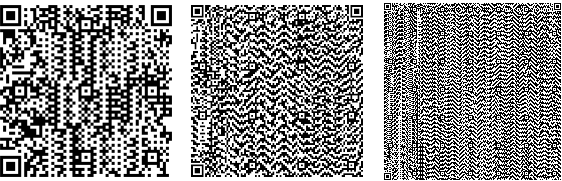
\includegraphics[width=9cm]{QRCodes.png}
\caption{QR code versions 10, 20, and 40 respectively.}
\end{figure}

\subsection{Research}
%SmartCards http://isrc.ccs.asia.edu.tw/www/myjournal/P013.pdf
%remote authentication usually uses smart cards or a mobile phone with QR codes
Work done in areas similar to mine have often had a slightly different focus. Before the prevalence of smartphones the focus was largely around the use of smartcards. \cite{SmartCards} A user would carry a smartcard with them which could be used to prove their identity to a computer before they entered their password. This is similar to how my system is going to work, but because my system uses a smartphone it is able to take advantage of the full range of features a smartphone can provide such as GPS, screen, and keyboard.

There has also been work done in regards to using QR codes for authentication. Like mine, these methods use QR codes to authenticate a user, but tend to have more of a focus on use as a one time pass. My system has Kerberos intergrated into the smartphone. This means that a user is able to log into their account and generate a QR code using their Kerberos ticket. The systems I have seen 
% cite some sources

\section{My Progress}
\subsection{Infrastructure} 
My current infrastructure involves two servers that are both running Ubuntu 14.04. The first server is used as the Kerberos key distribution center (KDC) running version 5 and a domain name server that uses Bind version 9 \cite{Bind}. The second server hosts an Apache web server which can be only be accessed with a valid Kerberos ticket from the KDC server. At the moment the Apache server is playing the role of any possible future Kerberos enabled service. It is a good service to use when testing because there is instant visual feedback when it is working. A use case that results in me being able to access the Apache server could be replaced with any other service such as SSH or access to my account from the user login GUI.

I am using Kerberos because it is runs on all popular operating systems and has built in support in a lot of existing services such as Apache, SSH, and Samba. This means that when a service is configured to connect with the user's KDC, they can use their TGT to access restricted web pages, ssh into protected machines, and access specific folders. I am using Kerberos version 5 because it is the most recent and has resolved some security concerns that were present in version 4 \cite{KerbUpdate}. Kerberos is also useful because all tickets have an expiry time. This is important in my system because if a malicious user intercepts the QR codes then they can only abuse the tickets in the short time window before they expire. Kerberos is single sign on which is useful in our QR code based system because the user can use the TGT to gain access to any new service they need without reentering their username and password. It is a protocol that is supported on all major operating systems and is well tested. If I was to try and design an authentication protocol myself it would require me to do all of the integration and testing which would take a long time without providing very much benefit.

In my project QR codes are going to be used as a primary communication channel between the user and their services. QR codes are a good option because they are easy to use, and hard to perform a man in the middle attack on. The malicious user would have to get a copy of all the user's QR codes before they could use them themselves.

Unfortunately QR codes do not have support direct binary encoding, this means that Kerberos tickets (which are stored in binary) need to be converted to an alphanumeric format before being encoded. I am currently converting the tickets to the string representation of hexadecimal but in the future I will convert them to base64 because it makes more use of the alphanumeric character set, allowing QR code sizes to be reduced further.

\subsection{Dynamic Grouping of Users}
Dynamic grouping of users is a concept which is used in two of my use cases. The idea is that a Kerberos enabled network has a set of groups with exclusive access to particular resources. A user needs to be a member of the group controling the resources before they are given access. Groups can be long lasting, but in my use cases I have designed them to be set up for short term interactions where users are given access to some resources for short periods to furfull a particular goal such as collaboration. At the end of the interaction e.g. working day or meeting, the group is cleared so that each time that group is used it has a fresh start and prevents users from accessing the resources outside of the intended times. Users are added to the group when they meet certain conditions e.g.\ they are in the meeting. Kerberos lacks native group control, so needs to be implemented by the service using Kerberos. My proposed system puts group support into Kerberos, then uses that to control when users can access particular resources. By having group support directly in Kerberos it creates a single point that needs to be changed, rather than having each resource controlling its own group independently.
%need to mention that there is no build in support for Kerberos groups at the moment

The point of the dynamic groups is that it gives the KDC a point of reference to see which users are currently meeting a certain condition. The condition could be a range of things, but in the case of my use cases they reflect the users location. The groups are designed for users to be added and removed from them frequently which differs from how groups usually operate in a Unix like system, where groups are infrequently added to or removed from. The group can be put in place for long term or short term activities depending on the resources a group is being given access to. A short term group can be set up for meetings so that anyone in the meeting gains access to a shared file system and printer so they can collaborate. A long term group could be set up for something like door access, you only want particular users to be able to open a certain door using their QR code.

%The idea of a dynamic group is that the user must perform an action which will get them added to the group, once they are in the group they have access to that groups resources, but will lose them again once they leave the group. How a user is added to a group can be done a number of different ways that I will go into shortly. Groups can be set up for meetings so that the users can access shared resources for the duration of the meeting, or could be used to ensure that the user can only log into a computer if they are in the room. By having these restrictions there is reduced risk of the users account, or resources being abused by a malicious user.

There are many ways of saying if a user is in the room or not, all are fit for different situations. The three main ways considered are: locating the user with Wi-Fi, GPS, and scanning of QR codes which will come in two forms; codes scanned an admin, and codes scanned by the user.

\begin{itemize}

\item Wi-Fi: It is possible to triangulate a user’s position using multiple Wi-Fi routers. As long as the user is connected to the systems Wi-Fi then their position can be worked out within X meters, which means that the system would be able to detect which room a user is in. The problem with this system is that it requires Kerberos to be integrated with the routers. It also means there needs to be a database of MAC addresses so that when a device is in range, the right user is associated with it. This means that a MAC address could be spoofed but the malicious user would have to spoof the MAC address, be in the right location, and have the victim users QR code tickets. This would be good for situations where a user needs to be confirmed to be in a room that does not need any kind of supervision.

\item GPS: GPS would would similar to Wi-Fi. The signal would have to be coming from a smartphone, and there would need to be a way of telling who was sending which GPS signal and it can happen automatically. It is not accurate indoors, so cannot be used to identify if a user is in a particular room. Another problem is that GPS can be easily spoofed, to be sure that the signal is correct, users of the system would need to be issued a GPS tracker which would syncronize directly with the KDC. By using the tracker the KDC knows it can trust the signal coming from it.

\item QR Code - User Scanned: When we need the user to prove they are in a particular room we can have them scan a room specific QR code which they scan after they have acquired their Kerberos ticket. The room specific code is combined with their ticket so that the the resource they are scanning their code at can see that they have both the rooms code and their ticket. This can be spoofable but if the room codes are changed enough then risk that they will be misused can be reduced.

\item QR Code - Admin Scanned: Used when access is being given to high value resources. The only way a user can get access to these is through the admin scanning their QR code. The idea is that these are often used for short term meetings where access to the resources is as limited as possible. The benefit of the admin having to scan the code also means that a meeting can take place with the admin being selective about who is given access rights to the meetings resources.

\end{itemize}


\subsection{Optimisation of QR Codes}
%todo actually get the version that was good
%todo reference 
The amount of information the QR codes can store increases as the version does. Kerberos tickets can be quite large so efficient storage is important. The amount of QR codes required to store the tickets needs to be small, but the speed and ease of scanning the QR codes also need to be taken into account. A high version code will store a lot, but it will also be hard to read. We can easily encode a whole ticket into a single QR code, but the resulting QR code is impractical to read, and impossible for a low resolution screen to display correctly. After performing some basic tests I was able to find a QR code version that allowed me to store the most information per code, while also being fast to read. Based on the size of my Kerberos TGT of X bytes, it would take X QR codes to encode it, each being scanned within a second by my smartphone.


\subsection{Transfer of a Login Session Use Case}
I am going to give a run through of my basic use case to show how a user’s ticket can be transferred from one machine to another using QR codes \footnotemark{YouTubeDemo}. Though basic, this use case shows that it is possible for a Kerberos ticket to be transferred between machines using QR codes. In the demo for this use case the QR codes are displayed on the computer screen, but an implemented version of this with a phone could display those QR codes on the phones screen to have the same effect. The process of this use case is outlined below:


\footnotetext{https://www.youtube.com/watch?v=v8ZZWC-jXeM\&list=UU3CfgH3Wtm0TTpxq0I92XFw}

\begin{itemize}
	\item Both computer A and B have no Kerberos tickets, and therefore are unable to access the Apache server.
	\item Computer A runs kinit which is a command line program used to authenticate a user to the Kerberos KDC and get their TGT. They enter their details and are given their TGT. They can then use this ticket to negotiate a ticket for the Apache server, granting them access to its resources.
	\item Computer A then runs the QR code creating program. The program takes the TGT from the ticket cache (the location Kerberos tickets are stored) and converts it to hex, it then takes the hex and splits it into small sections. Each of those sections are then encoded into a QR code with a number used to identify the order of the QR codes so they can be reassembled. 
	\item Computer B, which is running the QR code scanning software, scans each of the QR codes created by Computer A. When all the codes are decoded they are reassembled using the ordering numbers from before, converted back to binary, and then added to the Kerberos ticket cache. Computer B is now able to use the TGT just as Computer A could before to negotiate a ticket to access the Apache server.
	\item The tickets from computer A have now been transferred solely using QR codes as the primary means of communication.
\end{itemize}

If this was created, the use case would be carried out in a very similar way, but with computer A being replaced with an Android smartphone. The user would enter their login details into their phone which would create the QR codes for them to scan at any of the accepting systems, authenticating themselves to that system.

\subsection{Meeting Room Use Case}
In this use case, there is a meeting room with particular resources that users in the meeting need to access. Access should be easy for those in the meeting, but difficult for those outside of the meeting. Users get access to the resources such as a shared file system and printer server by being in the meeting room group. Each meeting has an admin who scans users Kerberos ticket QR codes as they enter. When a user enters or leaves the meeting room their QR codes are scanned to show this transition, and as a result they will be added or removed from the meeting room group. Users within the meeting can use the shared resources to collaborate from any of their Kerberos enabled devices. A malicious user in this use case would need to be physically present in the room. Kerberos tickets for these resources have a short lifespan, but can be renewed without a password prompt until the end of meeting. This means users in the room will be able to collaborate for the entire duration without reentering their password, but their device will have to keep renewing their ticket from KDC. Each time the ticket is renewed the KDC will check to see that the user is still part of the meeting group, if they are not then it will simply not give them the ticket they need for the resources, preventing the user from accessing them furthur.


\subsection{Proximity to Resources}
We want our users to only be able to use resources if they are actually in the geographical area of them. The phones GPS can be used to show were a user is, and such can be used to tell the KDC when the user is in or near the building with the resources. Users in the area are kept in a dynamic group so the KDC has an easy way of checking who can get tickets. This use case works in a very similar way to the meeting room, but rather than entering the particular room they are entering a certain proximity to the location of the resources. Since it is done with GPS is also means it can be done automatically. When a user tries to log in it polls their phone for their location, if they are in the locaton then they are added to the group, if they are not then they can not get the ticket. Since the users phone is tied to the KDC, it means that the KDC could inform the user that someone is attempting to access their account while they are out of the area. The problem with this use case is that the users GPS can not always be trusted, some versions of Android built around privacy are made to send incorrect GPS signals. To remedy this users can have a trusted device with them for the sole purpose of reporting their GPS signal. This means we can trust the GPS signal we are getting, but does also mean an increase in cost to the user. The GPS signal is weak indoors so can not be used to show that a user is in a particular room, but will be sufficient to show that a user is in or near the building.


\section{Related Work}
\subsection {Web Authentication Using A Mobile Phone}
This project allows a user to put a proxy between themselves and an untrusted computer for their websession \cite{Wu04secureweb}. The proxy server stores the usernames and passwords. A text message is used to authenticate the user's session to the proxy, and the proxy acquires the login sessions for the user so they do not have to enter their details on the suspicious computer.

My solution takes a different approach to this one, theirs can run on any computer because they just need to connect to their secure proxy. I sacrifice the ability to work anywhere for allowing more uses than just the web, and users of my program can transfer their permissions from one computer to another without having to enter their username and password again. 

\subsection{QR Code Based Door Access}
This project uses QR codes to open doors \cite{QRRelated}. The QR code does not expire which is dangerous, but it seems the main purpose of the project is for convenience over security. The idea behind their project is that a user can be emailed their access codes and seem intended to replace key cards. The problem with this method is that replay attacks could be set up to copy a user's QR code and give it to the attacker.

My implementation differs from this because rather than storing an access key, the QR codes in my system store the TGT which could be used to get the user a login session at a computer as well as room access. Their system sends QR codes via email. If someone was able to perform a man in the middle on their mailserver they could gain access to every QR code emailed out.


\section{Results}
Here I'm going to show the output of my programs. The output looks very similar to how the sequence diagrams look, with each action generating a line saying what it is doing. After looking at the results I will then explain how this improves on a use case that does not have access to my application.

\subsection{Meeting Room Results}
The above is an executed version of the use case using the proof of concept programs I have made. The user starts outside of the meeting room, they try and get their ticket, and the ticket check fails and the ticket is deleted. Next it is similated that they enter the room by scanning their QR code, they are then put into the meeting room group. When they try to get their ticket next it the check passes, allowing them to keep their ticket. They then use this ticket to SSH into the printer and the fileserver. SSH in this case takes to place of the two Kerberos enabled services, in the real version the user would actually check that they can print and access the file server. The user then leaves the room, when the user tries to refresh their ticket the KDC sees that they are no longer in the room and removes their ticket.

This is a use case that would be quite difficult without the intergration of groups into Kerberos and without the application use to scan users as they enter the room. If the grouping was not built into Kerberos then each service you wanted to restrict would need to have its own copy of the list of users, all requiring updates when a user is added or removed from the meeting room. You can also run into the possiablity that one of the services does not have a way of restricting access based on groups, so that would also need to be implemented. Without the application to scan users as they enter the room, the admin would have to manually enter the details of each person entering or leaving, it would also mean that the meeting room admin needs a full list of users to see if they were valid or not. By scanning a users QR code and checking in Kerberos to see if it is valid the admin is able to confirm that the person is a valid user with a resent Kerberos ticket.

\subsection{Proximity to Access Results}
In these results you can see what a user would expect to happen when they are using the system. To begin with the user is out of range, they then enter the area and it is shown that they are added into the dynamic group, next they try and get a ticket which they are granted because they are in the correct area they are granted the ticket. They then use the ticket to login and access the file server. They then log out and leave the area, removing them from the dynamic group. Next, a malicious user who knows that users details tries to login, when the check runs it sees that the user is not in the proximity of the building, so it can not be them logging in at this time, the KDC is able to make a note of this which can be forwarded to both the admin of the KDC and the user who's account has been compromised.

With this in place users are safe knowing that the only time someone can be on their account is when they are in the area. Any attempts to log into their account while they are away will generate a notification on their phone so they are aware of when they could be the target of a malicious user.

\subsection{How it Fits Together}
Above I have showcased how three different parts of the system could work. By combining these parts together it allows you to create a secure network with tight controls around users access to resources. It allows the user the security of never having to enter their password directly onto a computer because they can enter it into their phone and then use the QR codes on the phone to log them in by scanning it on the computer. This prevents them from keyloggers, the prevalence of Kerberos in the system also means that if an attack was to aquire the users ticket then they will only be able to use it for as long as the ticket is valid. By having them on smartphones it means that renewing a ticket is not very much effort for the user, so short ticket times are realistic.

%short ticket times, hard to steal QR codes, protect for resources using dynamic grouping for meetings, protection for users using the GPS stuff


\section{Problems Encountered}
Parts of the project did not go as planned. Overall this did not limit the knowledge that was gained from the project, does limit the useable applications created by the project. Before work could be started on the project I needed to set up the Kerberos infrastruture. My unfamiliarity with it meant that it took longer than expected, but a lot was learnt about Kerberos and how it would fit into the scope of the project. After better researching the Android application it was deceided that it was better of to implement a proof of concept rather than creating an actual application. This is because it made testing much faster as everything was contained within virtual machines, and it also meant that different use cases could be quickly prototyped using command line programs without having to worry about creating a GUI on an unfamiliar platform.

My checks to see if a ticket was valid all had to be client side. This is not optimal in a real system because it allows a malicious user to take their valid ticket before the check has taken place. Since my proof of concept assumes a non-malicious user it has not been a problem for my tests. Work on integrating it into MIT Kerberos would take a long time since it is a very large code base, so for my project I felt that showing how the system would work if implemented was enough.


\bibliographystyle{plain}
\bibliography{abibfile}

\end{document}